% LaTeX2e Template by Stephen Iota (https://stepheniota.github.io/)
% last updated: Oct. 2018

% for papers
%\documentclass[aps,onecolumn,superscriptaddress]{revtex4-1}
% https://www-d0.fnal.gov/Run2Physics/WWW/templates/revtex4.pdf
% https://cdn.journals.aps.org/files/revtex/auguide4-1.pdf
% for revTeX4-1 class options

% for other
\documentclass[12pt]{article}
\usepackage[margin=3.5cm]{geometry}

%%%%%%%%%%%%%%%%
%%% Packages %%%
%%%%%%%%%%%%%%%%

\usepackage[utf8]{inputenc}
\usepackage{amsmath}
\usepackage{amssymb}
\usepackage{amsfonts} % to remove math font when typesetting equations
\usepackage[thinc]{esdiff} 
\usepackage{graphicx}
\usepackage[shortlabels]{enumitem} % to change labels in enum/item
\usepackage[dvipsnames]{xcolor} % for colored links


% always put this at the end
\usepackage[
	colorlinks=true,
	citecolor=green!50!black,
	linkcolor=NavyBlue!75!black,
	urlcolor=green!50!black,
	hypertexnames=false]{hyperref} 

 
 %%%%%%%%%%%%%%%%%%
 %% New Commands %%
 %%%%%%%%%%%%%%%%%%
 
\newcommand{\email}[1]{\texttt{\href{mailto:#1}{#1}}}

\newcommand{\hint}[1]{\color{Blue}{#1}}
 
%----------------------------------------------------
%%%%%%%%%%%%%%%%%%
%% Front Matter %%
%%%%%%%%%%%%%%%%%%

%\pagenumbering{gobble} % no page numbers
\graphicspath{{figures/}} % set directory for figures
\usepackage{wrapfig}
%\setcounter{section}{-1} % start with section 0

%%%%%%%%%%%%%
%%% Title %%%
%%%%%%%%%%%%%
\begin{document}


\begin{center}

\Large{\textsc{Physics 40C:} Final Review}
\end{center}

\begin{center}
\large{December 7, 2018}	
\end{center}


%%%%%%%%%%
%% INFO %%
%%%%%%%%%%

%\begin{tabular}{rl}
%\textsc{SI Leaders}:
%&
%Urooza Ifran (\email{uifra001@ucr.edu})
%\&
%Stephen Iota (\email{siota001@ucr.edu})
%\\
%&
%Supplemental Instruction
%\\
%\textsc{Course}:
%&
%Physics 40C (Fall 2018), Prof.~Sales
%\\
%\textsc{Date}:
%&
%December 7, 2018
%\end{tabular}

%%%%%%%%%%%%%%
%% PROBLEMS %%
%%%%%%%%%%%%%%

%%%%%%%%%%%%%%%%%%%%%%%%%%%%%%%%%%%%%%%%%%%%%
%%% Magnetic Force between Parallel Wires %%%
%%%%%%%%%%%%%%%%%%%%%%%%%%%%%%%%%%%%%%%%%%%%%

\section{Magnetic Force between Parallel Wires}

Two long parallel wires, shown below, carry equal current in opposite directions.
\begin{enumerate}[(a)]
	\item Do the wires attract or repel each other? 
	\item What is the force between the wires?
\end{enumerate}

\begin{center}
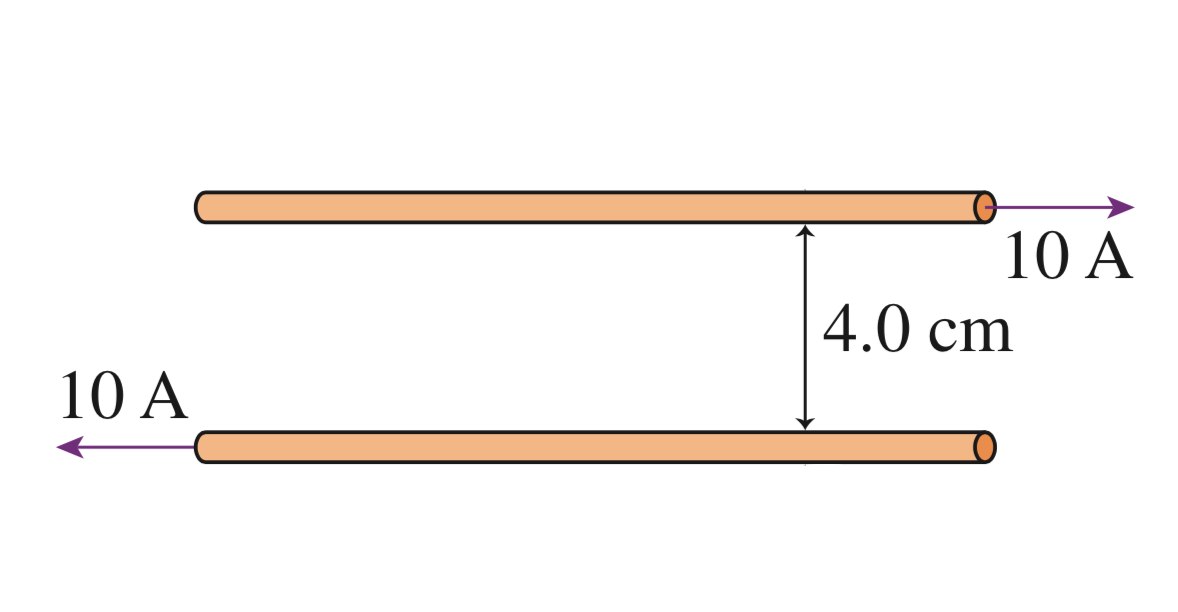
\includegraphics[width=.6\linewidth]{W7_3}
\end{center}



%%%%%%%%%%%%%%%%%%%%
%%% Faraday's Law $$
%%%%%%%%%%%%%%%%%%%%
\vspace{1in}
\section{Running to Create a Voltage}
You have a 2.5 m long antenna. How fast would you have to run with it to create 1.0 V potential using the Earth's magnetic field? $B_{\mathrm{Earth}}$ =  50 $\mu$T. 


\newpage
\section{Loop on the Moon}

From the moon, Earth's magnetic field can be approximated as a bar magnet. A loop is placed on the moon. The loop surface $S = 100$ m$^2$ is oriented \emph{tangentially} to the Moon's rotation. Estimate the current induced in the loop.
\vspace{2.5in}
\section{Combatting Faraday's Law}
A rectangular loop, laying in the xy plane, is subject to a perpendicular magnetic field $\vec{B} = 1 \hat{z}$ T. The loop's initial surface area $S = 20$ cm$^2$ is decreasing at a rate of 1 cm$^2/$s. We would like to keep the loop voltage-free. 

\begin{enumerate}[(a)]
	\item Phenomenologically, explain how you need to change the $\vec{B}$ field in order to keep the loop voltage-free.
	\item Make a guess as to what the solution, $\vec{B}(t)$, looks like. Should $\diff{\vec{B}}{t}$ be constant? If not, what should it depend on? Should the answer be exponential? Logarithmic? 
\end{enumerate}
%%%%%%%%%%
%%% LC %%%
%%%%%%%%%%

\newpage
\section{MRI Machines}

An MRI Machine needs to detect signals that oscillate at very high frequencies. It does so with an $LC$ circuit containing a 15 mH coil. To what value should the capacitance be set to detect a 450 MHz signal?


\vspace{2.5in}
\section{Phasors}

The emf phasor in the figure is shown at $t$ = 15.0 ms. 

\begin{enumerate}[(a)]
\item What is the angular frequency $\omega$? Assume this is the first rotation.
\item What is V($t=15$ms) if V$_0$ = 12 V?
\end{enumerate}
\begin{center}
	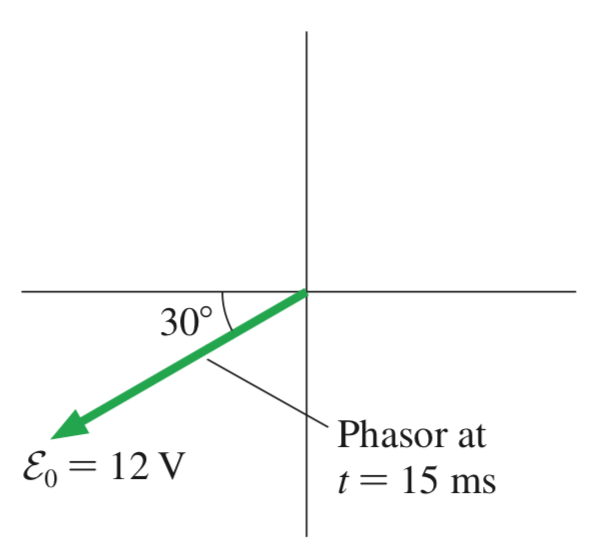
\includegraphics[width=.5\linewidth]{Final-fig2}
\end{center}


\newpage
\section{LC Switch Circuit}

The switch in the circuit below has been in position 1 for a long time. It is changed to position 2 at $t=0$ sec.

\begin{enumerate}[(a)]
	\item What is the maximum current through the inductor?
	\item What is the first time at which the current is maximum?
	\item Sketch plots of $Q(t)$ and $I(t)$. Explain why the current will never die out in an ideal $LC$ circuit. 
\end{enumerate}

\begin{center}
	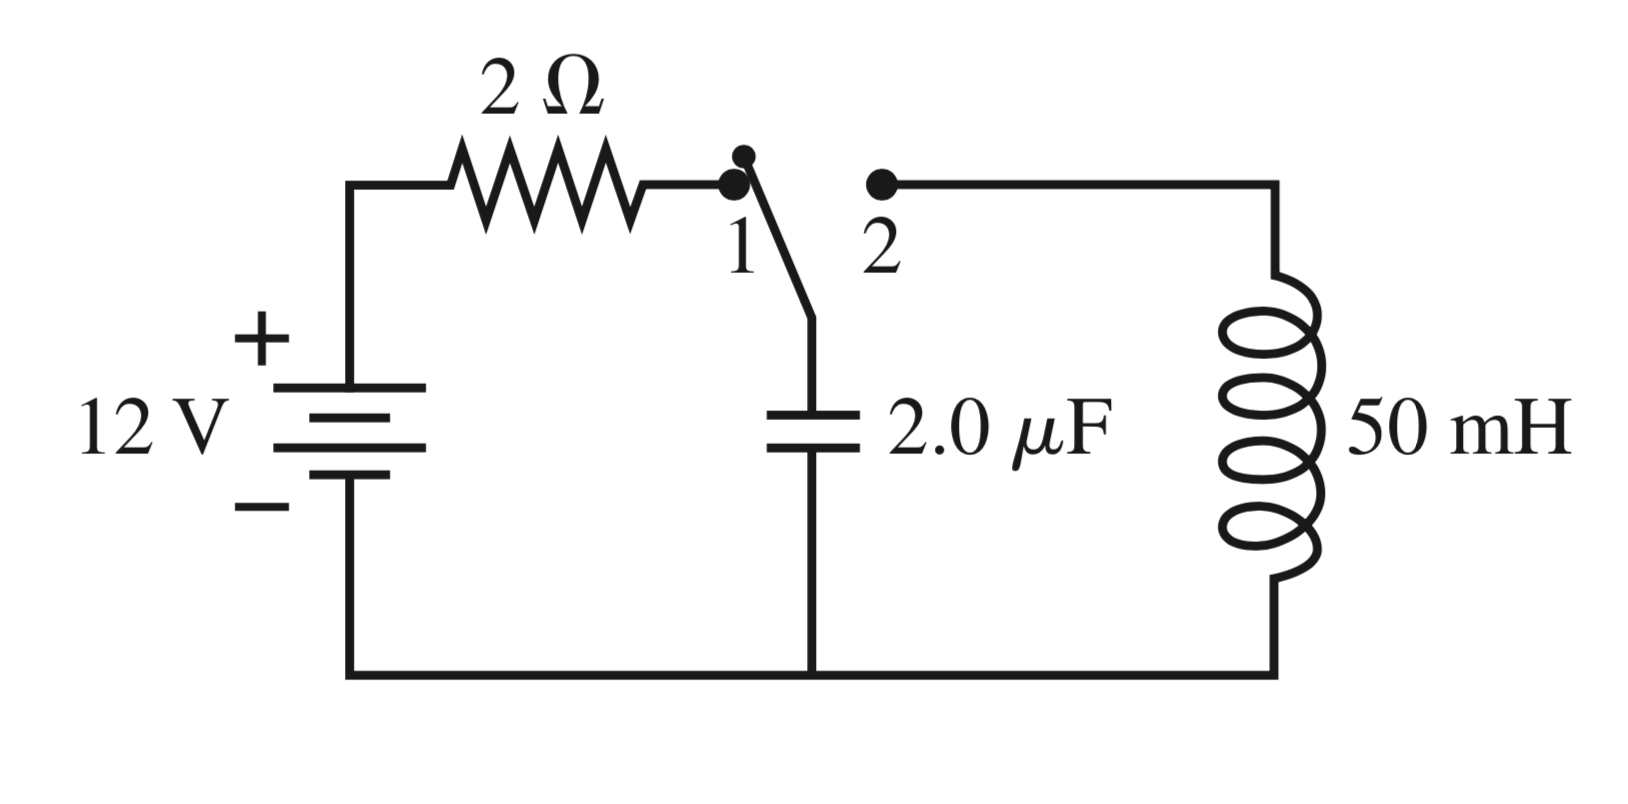
\includegraphics[width=.7\linewidth]{Final-fig3}
\end{center}

\vspace{1in}
\section{Building a Solenoid}
 You have a 1.0 m long copper wire. You want to make an $N$-turn current loop that generates a 1.0 mT magnetic field at the center when the current is 1 A. You must use the entire wire.
What will be the diameter of your coil?

\newpage
\section{Capacitor AC Circuit}

The peak current to and from a capacitor is 10 mA. What is the peak current if
\begin{enumerate}[(a)]
	\item The emf frequency is doubled?
	\item The emf peak voltage is doubled (at the original frequency)?
\end{enumerate}

\vspace{2in}
\section{Current Junction}


A wire carries current $I$ into the junction shown in the figure. What is the magnetic field at the dot?
\begin{center}
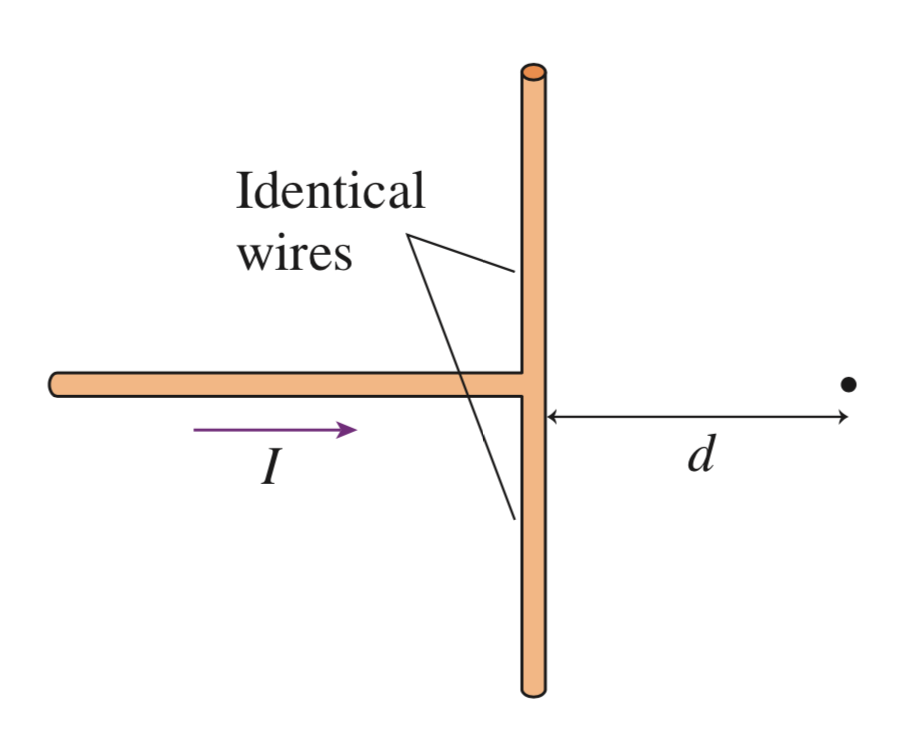
\includegraphics[width=.5\linewidth]{final-fig4}
\end{center}


\end{document}